\section{Cronograma}
\label{sec:cronograma}

El cronograma con los tiempo de desarrollo para cada una de las actividades se presenta en la Fig.~\ref{fig:cronogramalisto}. Para la ejecución del trabajo de grado se proponen cuatro etapas divididas en: evaluación del problema, simulación, desarrollo y experimentación. A continuación se detalla el proceso y los productos esperados en cada una de las actividades:


1. \textit{Identificar el estado de arte de la tomografía óptica coherente en aplicaciones biomédicas}. En este paso se busca crear un fundamento teórico y entendimiento del problema que se abordará en el trabajo de grado, lo cual se realizará mediante la lectura de artículos en revistas especializadas, tales como: \emph{Optics letters}\footnote{\url{https://www.osapublishing.org/ol/home.cfm}}, \emph{Biomedical optics express}\footnote{\url{https://www.osapublishing.org/boe/home.cfm}}, \emph{Journal of biomedical optics}\footnote{\url{https://spie.org/publications/journals/journal-of-biomedical-optics}}, \emph{Science}\footnote{\url{http://www.sciencemag.org/}}, entre otras del área óptica y biomédica. Con este proceso se entenderán conceptos fundamentales acerca del principio físico, funcionamiento y evolución de la tomografía óptica de coherencia. Esta faceta incluye la revisión constante de literatura para comprender y explicar los problemas que puedan surgir en etapas futuras.

2. \textit{Escribir anteproyecto del trabajo de grado}. Esta actividad busca obtener un documento resumen en el cual se plantea de manera clara el problema que se abordará para el trabajo de grado, en este busca depositarse el marco teórico y los conceptos básicos necesarios para el desarrollo del trabajo.


\begin{figure}[H]
	\centering
	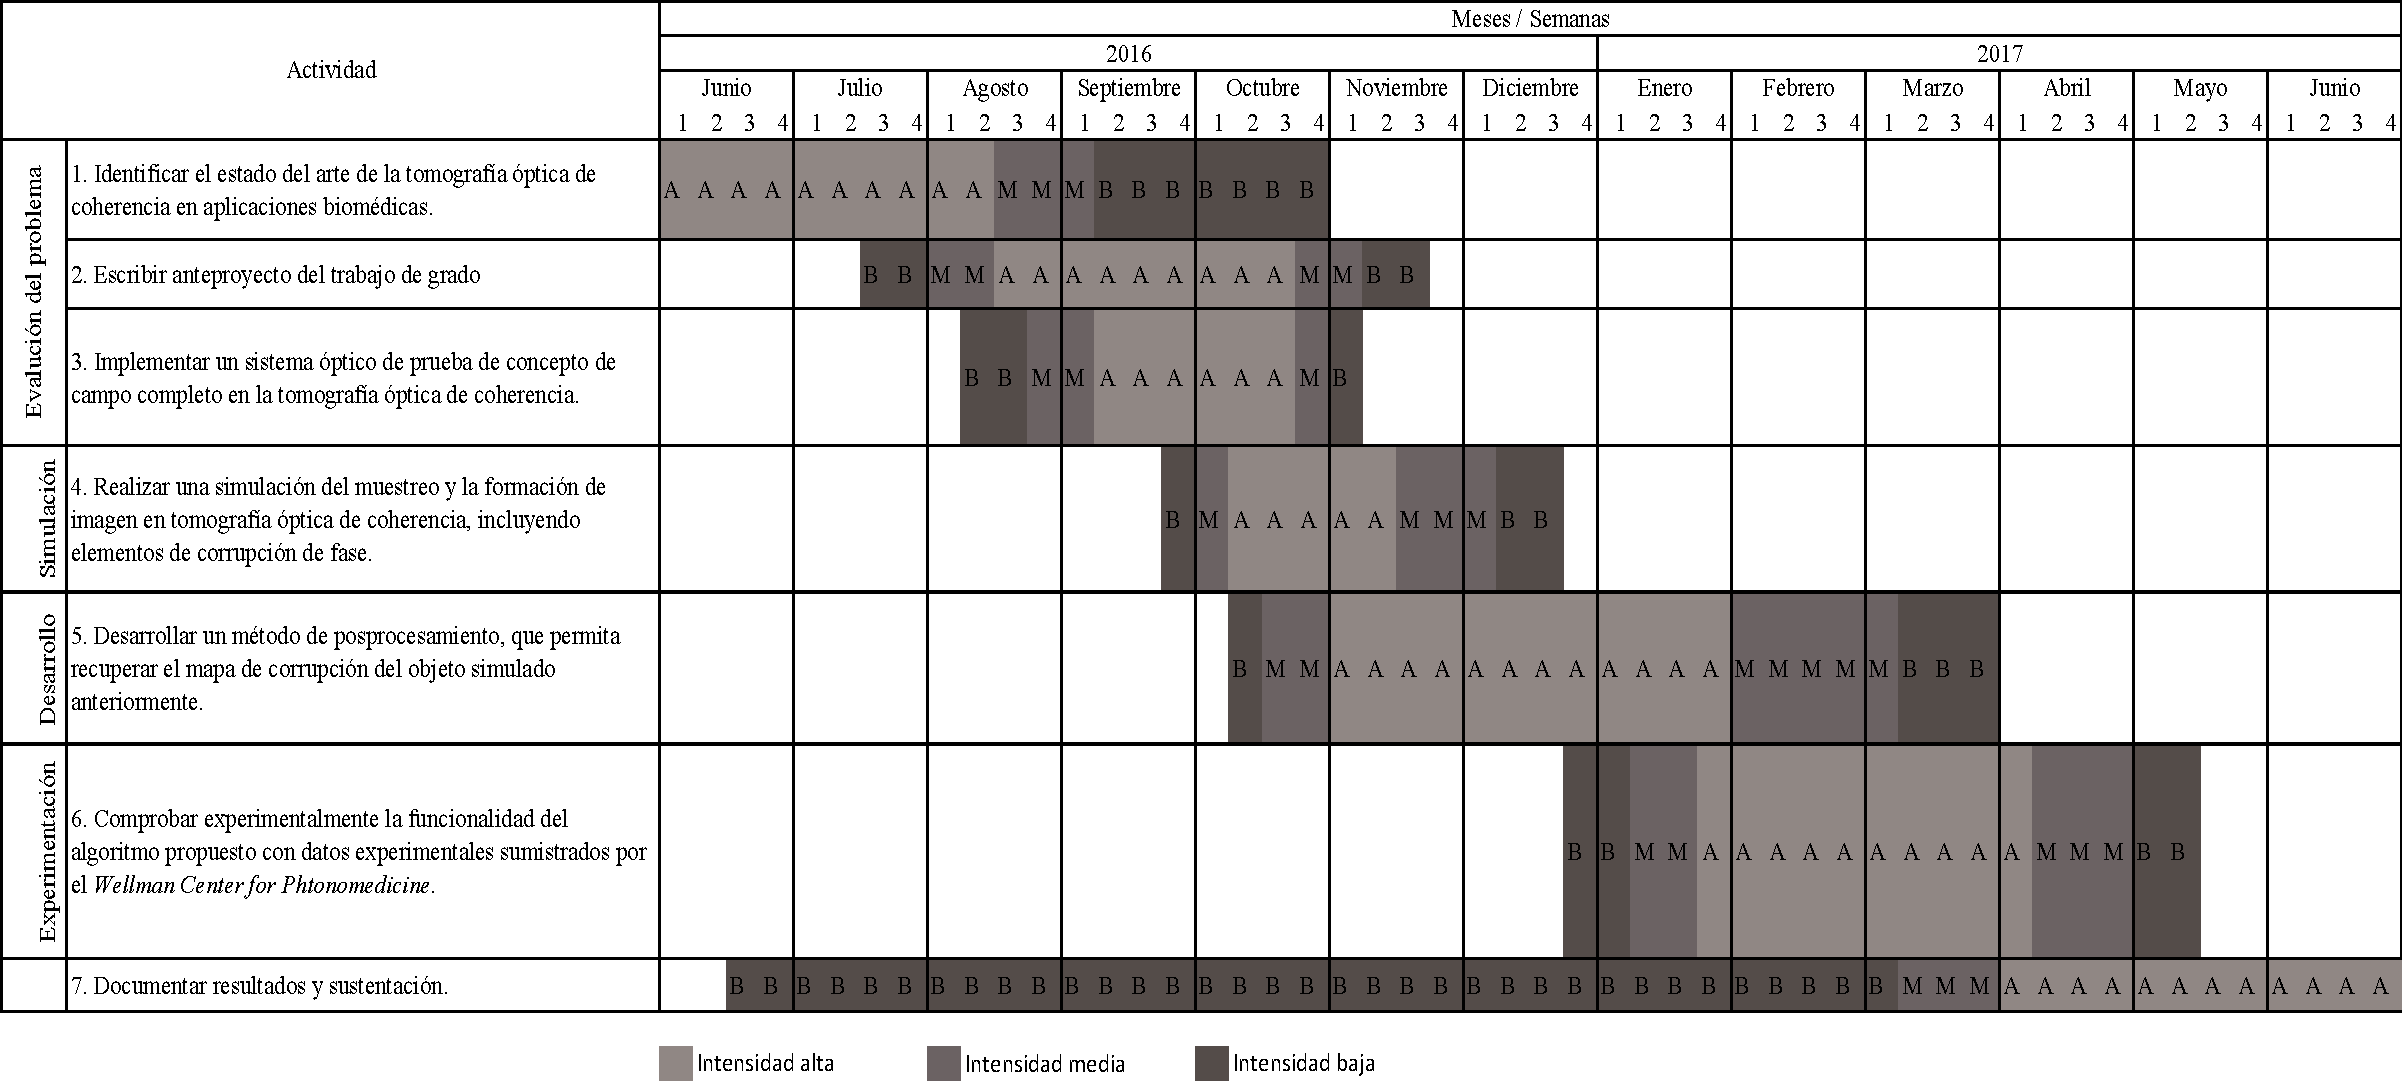
\includegraphics[scale=0.5, angle = 90]{Cronograma_listo.pdf}
	\caption[Cronograma de actividades.]{Cronograma de actividades.}
	\label{fig:cronogramalisto}
\end{figure}


3. \textit{Implementar un sistema óptico de prueba de concepto de campo completo en la tomografía de coherencia óptica}. Se implementará un interfómetro de Michelson con luz blanca, en donde el haz de referencia pueda ser desplazado con respecto al haz objeto, de esta manera se tendrá un sistema de OCT de primera generación con el cual se entenderán fenómenos y problemas que allí se presentan. A este sistema de OCT se le llama de campo completo debido a que la reflectividad de la luz en función de la profundidad es medida directamente para un plano usando una cámara CCD. En este montaje se planea utilizar dos objetos diferentes: el primer objeto que se empleará es un elemento traslucido con dos superficies, de forma que mediante el sistema de OCT se recuperará la separación entre las caras del objeto mediante la medición de la retroreflexión producida por el cambio del índice de refracción del medio. La segunda etapa consistirá en emplear un material traslucido y dispersivo, cuyas características se asemejen  a las muestras empleadas en OCT, de forma que mediante la retrodispersión producida por la muestra se obtendrá el mapa de reflectividad en función de la profundidad. 


4. \textit{Realizar una simulación del muestreo y la formación de imagen en tomografía óptica de coherencia, incluyendo elementos de corrupción de fase}. Esta etapa busca simular la formación de imagen en los sistemas de tomografía óptica de coherencia, mediante esta simulación se busca obtener un volumen de datos sobre los cuales se realizarán las primeras pruebas con los algoritmos desarrollados. En principio, se obtendrán datos para objetos conocidos empleando conceptos de OCT, luego computacionalmente se agregarán las características que poseen las imágenes obtenidas experimentalmente, esto incluye corrupciones en la fase por desalineamientos indeseados en la adquisición de las imágenes, así como la presencia de moteado por la dispersión de la luz. El objetivo final será poder reproducir mediante los algoritmos propuestos los mapas de corrupción que fueron añadidos en las imágenes.

5. \textit{Desarrollar un método de posprocesamiento que permita recuperar el mapa de corrupción de la imagen simulada anteriormente}. Con los datos simulados en el objetivo anterior, se desarrollará un algoritmo que permita encontrar los elementos de corrupción en la fase para el volumen de datos. La propuesta inicial consiste en emplear algoritmos de enfoque para medios turbios, en los cuales mediante posprocesamiento recuperan la fase que produce el mejor enfoque del haz cuando este se propaga en un medio turbio. De manera similar este concepto podría emplearse en OCT si se considera que cuando el haz de entrada posee un perfil gaussiano y adicionalmente la fase no está corrupta, el enfoque de este haz debe producir otro haz gaussiano, situación que no sucede cuando la fase está corrupta. Adicionalmente, consiste en la implementación de algoritmos que permitan la reducción de moteado, de forma que la fase pueda ser reconstruida de una manera más sencilla.

6. \textit{Comprobar experimentalmente la funcionalidad del algoritmo propuesto con datos experimentales suministrados por el \emph{Wellman Center for Photomedicine, Harvard Medical School and Massachusetts General Hospital}}. Los resultados obtenidos de las simulaciones se emplearán para corregir imágenes que provienen de datos experimentales de OCT, ya que en el laboratorio no se cuenta con un sistema de OCT de segunda generación que cumpla con las características requeridas para ser usado en pacientes, los datos serán suministrados por el co-asesor de este trabajo de grado. Con esto se espera validar los resultados obtenidos de manera experimental.

7. \textit{Documentación de resultados}. Los resultados serán de este trabajo de grado serán entregados a modo de documento, acompañado por la sustentación del mismo.

\section{Recursos}
\label{sec:recursos}

El desarrollo del trabajo de grado se realizará principalmente en el Laboratorio de Fotónica de la Universidad EAFIT que cuenta con los recursos e instrumentos necesarios para la realización de cada casi todas las actividades. Las implementaciones computacionales requieren de un equipo de computo con acceso a herramientas de programación tales como MATLAB, C++, Python y LabView;  de un sistema de computación en paralelo con arquitectura GPU y de los periféricos básicos, este sistema lo posee el Laboratorio de Fotónica. Para la realización del montaje de prueba, los instrumentos tales como la mesa óptica, espejos, divisores de haz, fuente de luz, piezoeléctricos y cámaras también se encuentran en las instalaciones del Laboratorio. El sistema de OCT que cumple con los requisitos de seguridad para la toma de muestras en pacientes, así como los componentes necesarios para la adquisición de datos y la toma de algunos datos, será realizada por el \emph{Wellman Center for Photomedicine}.

El recurso humano será aportado por las dos instituciones involucradas en este trabajo de grado, desde la Universidad EAFIT con el profesor e investigador René Restrepo quien será el asesor principal, desde el \emph{Wellman Center for Photomedicine} el Ph.D. Néstor Uribe-Patarroyo, se encargará también del asesoramiento en el desarrollo del trabajo de grado en calidad de co-asesor.